\documentclass{sigchi}

% Use this section to set the ACM copyright statement (e.g. for
% preprints).  Consult the conference website for the camera-ready
% copyright statement.

% Copyright
\CopyrightYear{2016}
%\setcopyright{acmcopyright}
\setcopyright{acmlicensed}
%\setcopyright{rightsretained}
%\setcopyright{usgov}
%\setcopyright{usgovmixed}
%\setcopyright{cagov}
%\setcopyright{cagovmixed}
% DOI
\doi{http://dx.doi.org/10.475/123\_4}
% ISBN
\isbn{123-4567-24-567/08/06}
%Conference
\conferenceinfo{CHI'16,}{May 07--12, 2016, San Jose, CA, USA}
%Price
\acmPrice{\$15.00}

% Use this command to override the default ACM copyright statement
% (e.g. for preprints).  Consult the conference website for the
% camera-ready copyright statement.

%% HOW TO OVERRIDE THE DEFAULT COPYRIGHT STRIP --
%% Please note you need to make sure the copy for your specific
%% license is used here!
 \toappear{
 A permissão para fazer cópias físicas ou digitais de parte ou todo o trabalho para uso pessoal ou em sala de aula é concedida gratuitamente, desde que tais cópias não passem a ser distribuídas para obtenção de lucro ou vantagem pessoal, e desde que todas as cópias ostentem este aviso e a citação completa na primeira página. Direitos reprográficos de outros para partes deste trabalho devem ser preservados. Qualquer outro tipo de reprodução requer permissão prévia ou pagamento de taxa. 
 
% Permission to make digital or hard copies of all or part of this work
% for personal or classroom use is granted without fee provided that
% copies are not made or distributed for profit or commercial advantage
% and that copies bear this notice and the full citation on the first
% page. Copyrights for components of this work owned by others than ACM
% must be honored. Abstracting with credit is permitted. To copy
% otherwise, or republish, to post on servers or to redistribute to
% lists, requires prior specific permission and/or a fee. Request
% permissions from \href{mailto:Permissions@acm.org}{Permissions@acm.org}. \\
% \emph{CHI '16},  May 07--12, 2016, San Jose, CA, USA \\
% ACM xxx-x-xxxx-xxxx-x/xx/xx\ldots \$15.00 \\
% DOI: \url{http://dx.doi.org/xx.xxxx/xxxxxxx.xxxxxxx}
 }

% Arabic page numbers for submission.  Remove this line to eliminate
% page numbers for the camera ready copy
% \pagenumbering{arabic}

% Load basic packages
\usepackage[brazil]{babel}
\usepackage[utf8]{inputenc}
\usepackage{balance}       % to better equalize the last page
\usepackage{graphics}      % for EPS, load graphicx instead 
\usepackage[T1]{fontenc}   % for umlauts and other diaeresis
\usepackage{txfonts}
\usepackage{mathptmx}
\usepackage[pdflang={pt-BR},pdftex]{hyperref}
\usepackage{color}
\usepackage{booktabs}
\usepackage{textcomp}

% Some optional stuff you might like/need.
\usepackage{microtype}        % Improved Tracking and Kerning
% \usepackage[all]{hypcap}    % Fixes bug in hyperref caption linking
\usepackage{ccicons}          % Cite your images correctly!
% \usepackage[utf8]{inputenc} % for a UTF8 editor only

% If you want to use todo notes, marginpars etc. during creation of
% your draft document, you have to enable the "chi_draft" option for
% the document class. To do this, change the very first line to:
% "\documentclass[chi_draft]{sigchi}". You can then place todo notes
% by using the "\todo{...}"  command. Make sure to disable the draft
% option again before submitting your final document.
% \usepackage{todonotes}

% Paper metadata (use plain text, for PDF inclusion and later
% re-using, if desired).  Use \emtpyauthor when submitting for review
% so you remain anonymous.

\def\plaintitle{E-Voz: melhorando a qualidade de decisões colaborativas para cidades inteligentes}
\def\plainauthor{Carlos Elmadjian, Tarcisio Pereira}
\def\emptyauthor{}
\def\plainkeywords{Fatores humanos; sistemas colaborativos; computação afetiva; cidades inteligentes}
\def\plaingeneralterms{Documentation, Standardization}

% llt: Define a global style for URLs, rather that the default one
\makeatletter
\def\url@leostyle{%
  \@ifundefined{selectfont}{
    \def\UrlFont{\sf}
  }{
    \def\UrlFont{\small\bf\ttfamily}
  }}
\makeatother
\urlstyle{leo}

% To make various LaTeX processors do the right thing with page size.
\def\pprw{8.5in}
\def\pprh{11in}
\special{papersize=\pprw,\pprh}
\setlength{\paperwidth}{\pprw}
\setlength{\paperheight}{\pprh}
\setlength{\pdfpagewidth}{\pprw}
\setlength{\pdfpageheight}{\pprh}

% Make sure hyperref comes last of your loaded packages, to give it a
% fighting chance of not being over-written, since its job is to
% redefine many LaTeX commands.
\definecolor{linkColor}{RGB}{6,125,233}
\hypersetup{%
  pdftitle={\plaintitle},
% Use \plainauthor for final version.
%  pdfauthor={\plainauthor},
  pdfauthor={\emptyauthor},
  pdfkeywords={\plainkeywords},
  pdfdisplaydoctitle=true, % For Accessibility
  bookmarksnumbered,
  pdfstartview={FitH},
  colorlinks,
  citecolor=black,
  filecolor=black,
  linkcolor=black,
  urlcolor=linkColor,
  breaklinks=true,
  hypertexnames=false
}

% create a shortcut to typeset table headings
% \newcommand\tabhead[1]{\small\textbf{#1}}

% End of preamble. Here it comes the document.
\begin{document}

\title{\plaintitle}

\numberofauthors{2}
\author{%
  \alignauthor{Carlos Elmadjian\\
    \affaddr{IME / USP}\\
    \affaddr{São Paulo, Brasil}\\
    \email{elmad@ime.usp.br}}\\
  \alignauthor{Tarcisio Pereira\\
    \affaddr{SIBiUSP}\\
    \affaddr{São Paulo, Brasil}\\
    \email{tarcisio1@hotmail.com}}\\
}

\maketitle

\begin{abstract}
  Utilizar tecnologias emergentes para melhorar a administração pública e tornar as cidades mais inteligentes é um fenômeno cada vez mais evidente. Mas quando utiliza-se dados fornecidos pelos usuários para esse fim, é preciso lidar com questões como o nível e qualidade da participação dos indivíduos para que iniciativas desse porte tenham sucesso. Este trabalho procura investigar se é possível melhorar a qualidade das contribuições colaborativas modificando interfaces convencionais, tanto com a adição de recursos que visam dar suporte a decisões mais conscientes dos cidadãos como também oferendo um padrão de interação que fomente sentimentos positivos nos usuários.
	
\end{abstract}

%\category{H.1.2.}{User/Machine Systems}{Human factors}
\category{H.5.2.}{User Interfaces}{Evaluation/methodology; Prototyping}
\keywords{\plainkeywords}

\section{Introdução}
O crescimento explosivo da Internet e do comércio eletrônico nos anos 1990 fez com que na última década houvesse uma pressão crescente sobre o setor público para o oferecimento de serviços eletrônicos aos cidadãos~\cite{tat:2002}, de modo a garantir maior comodidade, eficiência e transparência na relação entre representantes e representados. Tais serviços ficaram conhecidos como iniciativas \textit{e-governo}~\cite{carter:2005}.

Embora a ampla difusão e acesso a plataformas digitais no setor público seja um fenômeno inquestionável, sobretudo na América do Norte, Europa e leste asiático~\cite{nam:2011}, alguns autores ressalvam que poucas iniciativas desse porte conseguiram atingir um nível significativo de alcance e profundidade para que os cidadãos tenham a percepção de efetiva participação na administração pública~\cite{layne:2001}, seja pelo custo material e humano da infraestrutura tecnológica necessária para suportar essas iniciativas, seja pelo próprio desinteresse de agentes políticos.

\subsection{Ferramentas colaborativas}
Procurando preencher o vazio deixado por iniciativas \textit{e-governo} insatisfatórias, alguns aplicativos do setor privado têm surgido como um canal alternativo de comunicação entre cidadãos e representantes públicos. Várias dessas ferramentas têm um alcance municipal e utilizam-se de recursos interativos baseados na transparência dos problemas urbanos, uma condição fundamental para o aumento da confiança e adoção de novas tecnologias pelos indivíduos~\cite{carter:2005}.

Entre os principais aplicativos encontrados no mercado, podemos citar o Colab~\cite{colab:2016}, o Urbotip~\cite{urbotip:2016} e o Cidadera~\cite{cidadera:2016}. O típico modelo de negócio dessas ferramentas é estabelecer parcerias contratuais com prefeituras, oferecendo um canal direto de comunicação com o usuário que submete um problema à plataforma. Outra funcionalidade presente em todas as ferramentas do gênero é a possibilidade de os usuários votarem na resolução dos problemas que devem ser resolvidos com mais celeridade, dando suporte não só a causas pessoais como também coletivas. 

\subsection{Contribuição para cidades inteligentes}
Tanto a tarefa de reportar problemas quanto a de definição de prioridades podem fomentar o desenvolvimento de uma gestão mais moderna e eficiente das cidades. Dado que a maioria delas não conta com uma infraestrutura estática e pervasiva de sensores inteligentes, a utilização de agentes humanos em seu lugar não só parece ser uma solução mais econômica como também potencialmente mais refinada para o monitoramento urbano~\cite{zambonelli:2011}. 

No entanto, alguns autores alertam que há armadilhas nessa estratégia~\cite{irvin:2004, brabham:2009}, como: a) o aumento da descrença dos cidadãos, caso percebam que suas decisões estão sendo ignoradas; b) o aumento dos custos no processo decisório, onerando ainda mais o contribuinte; c) a possibilidade de uma má escolha coletiva cujo peso político não possa ser ignorado; d) a desconsideração da opinião de especialistas. Ainda assim, há diversas evidências sustentando que o resultado das interações colaborativas tende a ser majoritariamente positivo~\cite{schuurman:2012}.

\section{Características da interação}
Embora o benefício potencial dessas ferramentas seja patente, é possível identificar, no entanto, alguns problemas quanto ao seu uso e experiência de usuário. Um dos primeiros é a baixa adesão, participação e representatividade dos usuários. Se um aplicativo desse tipo é capaz de mobilizar apenas um perfil muito específico de usuário, pertencente a um determinado estrato social, há um possível esvaziamento da legitimidade da plataforma.

Outro entrave é que o ambiente de participação em tecnologias emergentes como essa favorece o que alguns autores chamam de libertarianismo individualista~\cite{brabham:2008} e, portanto, ainda que se argumente em favor da \textit{sabedoria das multidões}~\cite{surowiecki:2005}, observa-se uma tendência de os usuários reportarem problemas e apoiarem soluções que vão ao encontro apenas dos seus próprios interesses.

Desse cenário decorre ainda uma outra questão pertinente à área de Interação Humano-Computador, que é a criação de um vínculo emocionalmente negativo na interação entre os usuários e os aplicativos do gênero. Muitos indivíduos recorrem a essas ferramentas como uma válvula de escape para frustrações com a cidade e os representantes públicos. Já os eventuais relacionamentos entre os usuários nas plataformas acaba por estimular uma espiral de negatividade~\cite{slater:2007} sobre as questões municipais. Uma das possíveis consequências disso é a proliferação de tomadas de decisão de baixa qualidade, caracterizadas pela celeridade e forte conteúdo emocional, no lugar de critérios racionais de utilidade~\cite{tversky:1986}.

\begin{figure}
	\centering
	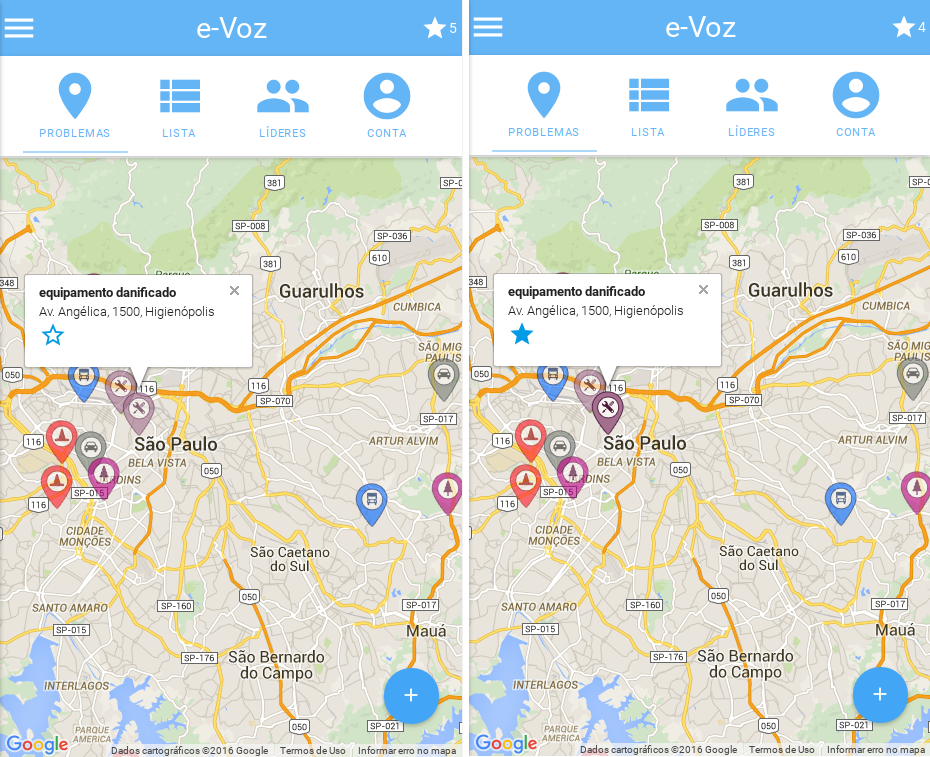
\includegraphics[width=0.85\columnwidth]{figures/prototipo1a}
	\caption{Demonstração do processo de escolha dos problemas prioritários: o usuário seleciona um \textit{pin} no mapa e usa uma das suas estrelas disponíveis (canto esquerdo superior) para marcar o problema. }~\label{fig:figure1}
\end{figure}

\section{A ferramenta e-Voz}
Para investigar se com alterações em recursos interativos é possível identificar melhorias na qualidade das decisões colaborativas e no vínculo afetivo do usuário com aplicações do gênero, desenvolvemos o conceito de um aplicativo denominado \textit{e-Voz}, capaz de emular tarefas semelhantes àquelas propostas pelas ferramentas já citadas.

A ideia por trás do \textit{e-Voz} é oferecer uma plataforma que em termos funcionais seja indistinta das demais, mas que do ponto de vista da experiência de usuário possa fomentar a participação, sentimentos positivos e a conscientização sobre os problemas da cidade, na expectativa de que o usuário possa estabelecer um comportamento mais colaborativo com o município.

\begin{figure}
	\centering
	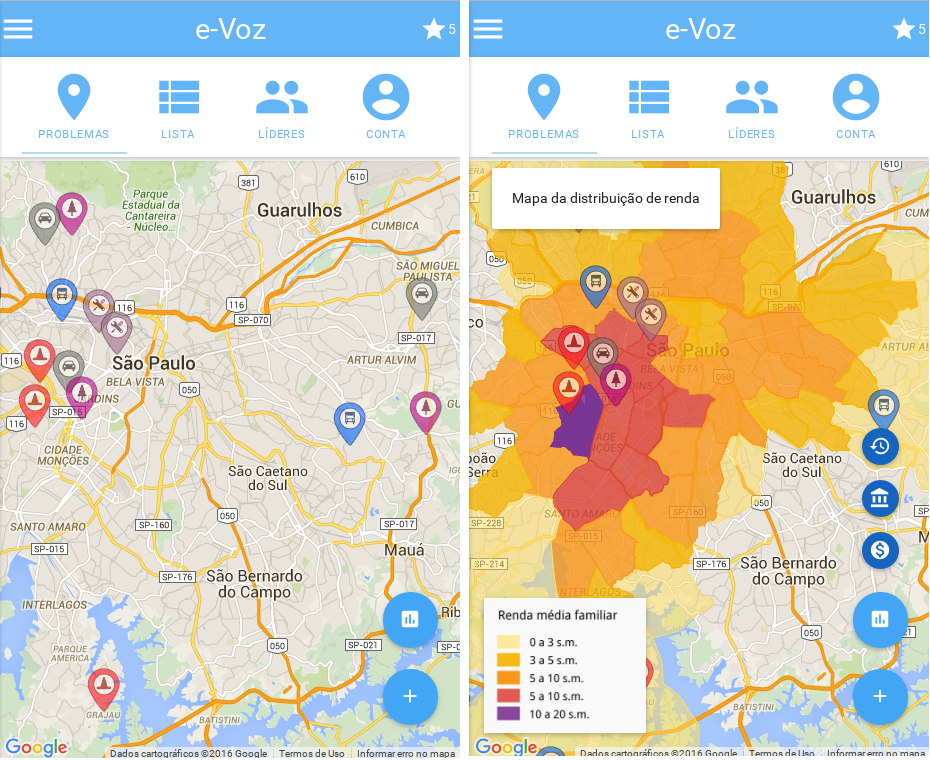
\includegraphics[width=0.85\columnwidth]{figures/prototipo2b}
	\caption{Ao selecionar o botão de auxílio com dados estatísticos, três opções de camadas de dados sobre o mapa se tornam disponíveis: frequência de ocorrências reportadas nos últimos seis meses, taxa de resolução dos problemas pela Prefeitura de São Paulo e distribuição de renda familiar (tela à direita).  }~\label{fig:figure2}
\end{figure}

Por isso, consideramos relevante dar destaque para o recurso de escolher incidentes que devem ser resolvidos mais rapidamente pela Prefeitura (Figura~\ref{fig:figure1}). A ideia é que o usuário se sinta um agente participativo na resolução dessas questões e não um mero fiador de reclamações. Para auxiliá-lo na tomada de decisão, adicionamos um botão que exibe algumas estatísticas fictícias sobre a cidade (Figura~\ref{fig:figure2}), um recurso ausente em outras ferramentas similares.


Para o estimular participação dos usuários, procuramos também utilizar técnicas de gamificação~\cite{deterding:2011}, como um \textit{ranking} dos membros mais colaborativos, inserção de insígnias e troféus, com o cuidado de não salientar a competitividade, mas a colaboração entre os usuários. Contudo, no escopo deste trabalho, investigamos somente os aspectos afetivos da interação e suas consequências na qualidade das decisões. 


\section{Materiais e métodos}
Dois protótipos distintos baseados no conceito proposto foram desenvolvidos para o estudo, utilizando as tecnologias HTML5, JavaScript, CSS3 e a \textit{Application Programming Interface} (API) para mapas do Google~\cite{googlemaps:2016}, sendo posteriormente compilados para a plataforma Android por meio do \textit{framework} Apache Cordova~\cite{cordova:2016}. Para o experimento com usuários, foi utilizado um aparelho Motorola Moto G Dual SIM, com uma tela de 4,5 polegadas.

\subsection{Design experimental}
Para esta investigação, propusemos um teste A/B com os participantes entre os dois protótipos, de modo que a única diferença visual entre ambos seria o botão adicional de recursos estatísticos, presente na segunda versão (conf. Figura~\ref{fig:figure1} e Figura~\ref{fig:figure2}). Desse modo, procurou-se minimizar a possibilidade de que outras variáveis relativas ao experimento tivessem algum impacto deletério sobre os resultados.

No teste proposto, os indivíduos deveriam completar a mesma tarefa com cada versão e, ao final cada uma, responder a um questionário com quatro questões cujas respostas foram dispostas em uma escala de Likert de cinco níveis, com o intuito de verificar qual a experiência de usuário obtida. Para evitar vieses relacionados à ordem de execução das tarefas, metade dos voluntários deveria interagir primeiro com a versão I e a outra metade com a versão II.

Optou-se por realizar uma investigação inteiramente intra-sujeito e sem comparação com outras ferramentas equivalentes, a fim eliminar o viés de confirmação tipicamente presente em experimentos dessa natureza~\cite{dell:2012}. Após a conclusão das tarefas, uma entrevista semiestruturada deveria se realizada com cada participante a fim de identificar o cumprimento ou não de critérios de experiência de usuário, registrar os sentimentos relatados, investigar eventuais mudanças de comportamento na interação com cada protótipo e coletar opiniões gerais sobre a ferramenta.

\subsection{Procedimento experimental}
Todos os participantes se sujeitaram ao experimento em ambientes naturais, receberam informações sobre natureza da investigação, a garantia do experimentador de que todas as informações colhidas seriam confidenciais e o compromisso de que ele poderia desistir do experimento a qualquer momento que desejasse.

Uma vez de acordada sua participação, o experimentador exibia ao voluntário um dos protótipos da ferramenta \textit{e-Voz}, mostrando todas as suas telas e recursos interativos para que o participante pudesse se familiarizar com o aplicativo. Durante essa etapa, ele também era instruído sobre o contexto em que estava inserida a ferramenta e qual seria a natureza da tarefa requisitada, isto é, definir cinco problemas como prioritários dentre os 15 dispostos sobre o mapa do aplicativo com o intuito de auxiliar a Prefeitura de São Paulo na alocação de recursos públicos, utilizando ou não o botão de auxílio estatístico (no caso da versão II).

Havia cinco categorias diferentes de problemas e eles foram distribuídos sobre o mapa de modo que houvesse pelo menos um de cada tipo em áreas menos assistidas pelo poder público --- segundo as estatísticas fornecidas. O objetivo dessa configuração era salientar a existência de opções aparentemente mais justas do ponto de vista administrativo.

Enquanto o usuário selecionava os problemas que na sua opinião eram prioritários, o experimentador cronometrava o tempo gasto com a tarefa. Finda essa etapa, o participante recebia o questionário. O mesmo procedimento era adotado então com a outra versão da ferramenta.

Concluída essa etapa, o experimentador passava a fazer algumas questões abertas pré-definidas ao usuário, bem como outras perguntas que o experimentador julgasse pertinente no contexto, tanto para clarificar uma resposta dada quanto para dirimir dúvidas sobre o comportamento observado do participante.


\section{Resultados}
Participaram do experimento 11 voluntários --- oito homens e três mulheres --- todos entre 26 e 41 anos, sendo sete deles moradores da zona oeste da cidade de São Paulo. A ocupação predominante entre os participantes foi de estudante de ensino superior (cinco, ao todo). Para a condução do experimento, seis voluntários iniciaram primeiro sua interação com o protótipo I e depois com II, enquanto cinco procederam de forma inversa.

\begin{table}
	\centering
	\begin{tabular}{l r r}
		% \toprule
		\multicolumn{3}{c}{\small{\textbf{Resultados}}} \\
		\midrule
		{\small\textit{Métrica}}
		& {\small \textit{Protótipo I}}
		& {\small \textit{Protótipo II}} \\
		\midrule
		Tempo médio gasto no experimento & 145,8 s & 81,8 s\\
		Facilidade de completar a tarefa & 90,9 \% & 63,6 \%\\
		Sentimentos positivos com a tarefa & 81,8 \% & 90,9 \% \\
		Sentiu-se envolvido com a cidade & 72,7 \% & 72,7 \%\\
		Sentiu-se motivado a participar mais & 81,8 \% & 81,8 \%\\
		Preferência de uso & 27,3 \% & 72,7 \%\\
		% \bottomrule
	\end{tabular}
	\caption{Principais resultados quantizados colhidos a partir dos questionários e entrevista.}~\label{tab:table1}
\end{table}

A Tabela~\ref{tab:table1} condensa os principais resultados obtidos no experimento. De modo geral, a maioria dos participantes (72,7 \%) preferiu a versão II, cerca de 63,6 \% consideraram o recurso de auxílio útil à tarefa, nenhum participante considerou que esse recurso atrapalha a sua realização e, em média, uma quantidade de tempo significativamente maior de tempo foi gasta com a segunda versão.

Em termos de comportamento, observou-se que os participantes mostraram uma tendência em priorizar a solução de problemas mais próximos à sua residência ou local de trabalho usando o protótipo I. Já entre os quatro voluntários que não verificaram utilidade no recurso de auxílio, três sequer interagiram com ele.

Não houve diferença entre os protótipos I e II quanto à motivação e envolvimento dos usuários. Em torno de 81,8 \% dos voluntários disseram estar motivados a continuar utilizando a plataforma e 72,7 \% afirmaram se sentirem envolvidos com a cidade no processo de decisão. No entanto, em relação aos aspectos afetivos, houve uma clara distinção entre as duas versões: todos os usuários que preferiram o protótipo II relataram sentimentos mais positivos de solidariedade, confiança, justiça ou conscientização em comparação com a versão I. Por outro lado, alguns participantes consideraram que a tarefa se torna mais difícil de concluir com o auxílio estatístico.


\section{Discussão}
Os dados reforçam a hipótese do viés de disponibilidade~\cite{tversky:1973} na tomada de decisão dos participantes. No grupo que interagiu primeiro com o protótipo I e depois com o II, nota-se uma alteração no critério de escolha da prioridade dos problema com o aumento de informações que subsidiam a tarefa. O mesmo não se observa no grupo que inicia a interação pelo protótipo II e depois segue para o I. Quando questionados sobre a mudança de postura, a maior parte dos participantes reconheceu utilizar um critério individualista quando não havia informações estatísticas disponíveis sobre a cidade, o que parece indicar que o recurso impacta positivamente para a tomada de decisões mais coletivistas.

As pessoas que efetivamente usaram os recursos adicionais levaram mais tempo para concluir a sua escolha. Tal demora pode ser justificada com a quantidade maior de informação oferecida, que acabou demandando ``mais reflexão'', segundo muitos voluntários. Também houve uma forte correlação entre a percepção de utilidade do recurso de auxílio e o tempo gasto para realizar a tarefa: aqueles que consideraram tal recurso irrelevante foram consistentemente mais rápidos que os demais, dando fôlego à hipótese de pré-julgamento na qualidade das decisões~\cite{tversky:1986}.

Não cabe ao escopo deste trabalho discutir as consequências sociais de decisões mais coletivista que individualistas (é possível citar exemplos de sociedades prósperas em ambos os casos), mas há sólidas evidências de que o comportamento solidário se traduz em mais bem-estar individual~\cite{thoits:2001}. Muitos usuários confirmaram que sentiram mais altruístas, confiantes e comprometidos com a cidade de São Paulo utilizando a versão II. Alguns chegaram até a argumentar que poderiam embasar melhor ainda sua decisão com outros dados estatísticos não providos pela ferramenta, o que indica um nível de engajamento não observado na interação com o protótipo I.


%\section{Limitações e trabalhos futuros}
%Não está claro ainda se a percepção de um comportamento solidário por parte dos usuários se deve à ordem com que os protótipos I e II foram apresentados. Entre aqueles que começaram pela segunda versão e utilizaram os dados estatísticos, não houve um juízo de altruísmo sobre a qualidade da decisão, embora esses participantes tenham reconhecido a utilidade do recurso de auxílio para a tarefa. Portanto, para dirimir dúvidas dessa natureza, é necessário um estudo com um número maior e mais heterogêneo de participantes.
%
%É preciso também investigar outras características incutidas nos protótipos para melhorar a participação dos usuários, como os recursos de gamificação e elementos de rede social. Tal pesquisa é necessária, sobretudo, para verificar se esses recursos têm um efeito duradouro na aderência dos usuários à plataforma ou não, algo que não está claro na literatura~\cite{hamari:2014}.


\section{Conclusão}
Oferecer recursos para a melhoria de decisão em plataformas colaborativas sem onerar a usabilidade de interfaces pode inicialmente ser um desafio, mas os efeitos aparentes tanto na qualidade da interação (percepção dos usuários) quanto na utilidade parecem indicar um benefício significativo tanto aos usuários quanto à atividade-fim dessas ferramentas.


\section{Agradecimentos}

Agradecemos a todos os participantes que se submeteram voluntariamente ao experimento e aos nossos revisores, com seus comentários e críticas valiosas para o trabalho.


\balance{}


% BALANCE COLUMNS
\balance{}

% REFERENCES FORMAT
% References must be the same font size as other body text.
\bibliographystyle{SIGCHI-Reference-Format}
\bibliography{sample}

\end{document}

%%% Local Variables:
%%% mode: latex
%%% TeX-master: t
%%% End:
